
\Opensolutionfile{ans}[ans/ansTN]	
\noindent\textbf{PHẦN I.} Thí sinh trả lời từ câu 01 đến câu 12. Mỗi câu hỏi thí sinh chỉ chọn một phương án.
\Opensolutionfile{ans}[ans/ansTN]	
\noindent\textbf{PHẦN I.} Thí sinh trả lời từ câu 01 đến câu 12. Mỗi câu hỏi thí sinh chỉ chọn một phương án.

\begin{ex}%[NB]
    Xét hai đại lượng $x$, $y$ phụ thuộc vào nhau. Trường hợp nào sau đây thì $y$ là hàm số của $x$?
    \choice
    {\True $y = 8x^2$}
    {$\dfrac{x^2}{25} + \dfrac{y^2}{16} = 1$}
    {$y^2 = 8x$}
    {$(x-2)^2 + (y+3)^2 = 4$}
    \loigiai{
    Theo định nghĩa, $y$ là hàm số của $x$ nếu với mỗi giá trị của $x$ xác định duy nhất một giá trị của $y$.

    \begin{itemize}
        \item Với $y=8x^2$, mỗi giá trị của $x$ cho duy nhất một giá trị của $y$.
        
        \item Với $\dfrac{x^2}{25}+\dfrac{y^2}{16}=1$, khi $x=0$ thì $y=\pm 4$.
        
        \item Với $y^2=8x$, khi $x=2$ thì $y=\pm 4$.
        
        \item Với $(x-2)^2+(y+3)^2=4$, đây là phương trình đường tròn nên có những giá trị $x$ ứng với hai giá trị $y$.
    \end{itemize}

    Vậy đáp án đúng là:
    $$
    y=8x^2.
    $$
    }
\end{ex}

\begin{ex}%[NB]
    \immini{
        Cho đồ thị của một hàm số bậc hai như hình bên. Trong các khẳng định sau, khẳng định nào đúng?
        \choice
        {Trên khoảng $(2;+\infty)$ hàm số đồng biến}
        {Trên khoảng $(2;+\infty)$ hàm số nghịch biến}
        {Trên khoảng $(-\infty;2)$ hàm số nghịch biến}
        {\True Trên khoảng $(-\infty;2)$ hàm số đồng biến}
    }{
    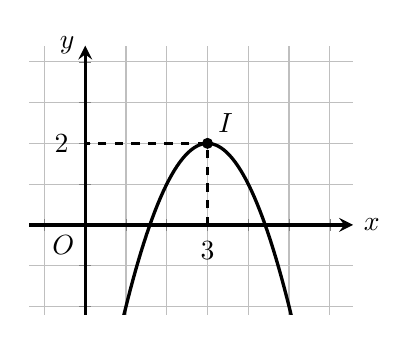
\begin{tikzpicture}
    \begin{axis}[
        scale=.6,
        xlabel={$x$},
        ylabel={$y$},
        axis lines=middle,
        line width=1.2pt,
        grid=major,
        xmin=-1.2, xmax=6.4,
        ymin=-2.2, ymax=4.4,
        axis equal,
        xtick={-2,-1,0,1,2,3,4,5,6},
        ytick={-2,-1,0,1,2,3,4,5},
        xticklabels={,,,,,$3$},
        yticklabels={,,,,$2$},
        xlabel style={at={(ticklabel* cs:1)}, anchor=west},
        ylabel style={anchor=east},
        y tick label style={anchor=east},
    ]
    \addplot[domain=-1.2:5.5, samples=100, color=black, very thick]{-(x-3)^2 +2};

    \fill (axis cs: 3,2) circle (2pt); 
    \node at (axis cs: 3,2) [above right] {$I$}; 

    \draw[very thick, dashed] (axis cs: 3,0) -- (axis cs: 3,2) -- (axis cs: 0,2);

    \node at (axis cs:0,0) [below left] {$O$};
    \end{axis}
    \end{tikzpicture}
    }
    \loigiai{
    Từ đồ thị ta thấy parabol có đỉnh $I(3;2)$ và quay bề lõm xuống dưới.

    Do đó:
    \begin{itemize}
        \item Hàm số đồng biến trên khoảng $(-\infty;3)$.
        \item Hàm số nghịch biến trên khoảng $(3;+\infty)$.
    \end{itemize}

    Suy ra trên khoảng $(-\infty;2)$ hàm số đồng biến.

    Vậy đáp án đúng là:
    ``Trên khoảng $(-\infty;2)$ hàm số đồng biến''.
    }
\end{ex}

\begin{ex}%[NB]
    Cho tam thức bậc hai $f(x) = - x^2 + 3x - 2$ có đồ thị là parabol $(P)$. Trục đối xứng của $(P)$ là đường thẳng nào sau đây?
    \choice
    {$x = \dfrac{2}{3}$}
    {$x = -20$}
    {$x = 3$}
    {\True $x = \dfrac{3}{2}$}
    \loigiai{
    Với hàm số bậc hai:
    $$
    y=ax^2+bx+c,
    $$
    trục đối xứng là:
    $$
    x=-\dfrac{b}{2a}.
    $$

    Ở đây:
    $$
    a=-1,\quad b=3.
    $$

    Suy ra:
    $$
    x=-\dfrac{3}{2(-1)}=\dfrac32.
    $$

    Vậy trục đối xứng là:
    $$
    x=\dfrac32.
    $$
    }
\end{ex}

\begin{ex}%[NB]
    Trong mặt phẳng toạ độ $Oxy$, cho đường thẳng $d \colon x - 2y + 2026 = 0$. Trong các vectơ sau, vectơ nào \textbf{không phải} là một vectơ pháp tuyến của $d$?
    \choice
    {$\overrightarrow{m} = (1;-2)$}
    {\True $\overrightarrow{n} = (2;1)$}
    {$\overrightarrow{p} = (2;-4)$}
    {$\overrightarrow{q} = (-3;6)$}
    \loigiai{
    Đường thẳng:
    $$
    d:x-2y+2026=0
    $$
    có một vectơ pháp tuyến là:
    $$
    (1;-2).
    $$

    Các vectơ cùng phương với $(1;-2)$ đều là vectơ pháp tuyến của $d$.

    \begin{itemize}
        \item $(2;-4)=2(1;-2)$ nên là vectơ pháp tuyến.
        
        \item $(-3;6)=-3(1;-2)$ nên là vectơ pháp tuyến.
        
        \item $(2;1)$ không cùng phương với $(1;-2)$.
    \end{itemize}

    Vậy vectơ không phải vectơ pháp tuyến là:
    $$
    (2;1).
    $$
    }
\end{ex}

\begin{ex}%[NB]
    Trong mặt phẳng toạ độ $Oxy$, cho đường thẳng $\Delta \colon 2x + 3y - 5 = 0 $. Trong các đường thẳng sau, đường thẳng nào song song với $\Delta$?
    \choice
    {$d_1 \colon 4x - 6y + 10 = 0$}
    {\True $d_2 \colon -4x - 6y - 5 = 0$}
    {$d_3 \colon 4x + 6y - 10 = 0$}
    {$d_4 \colon 6x + 4y + 10 = 0$}
    \loigiai{
    Hai đường thẳng:
    $$
    a_1x+b_1y+c_1=0,\quad a_2x+b_2y+c_2=0
    $$
    song song khi:
    $$
    \dfrac{a_1}{a_2}=\dfrac{b_1}{b_2}\ne\dfrac{c_1}{c_2}.
    $$

    Với:
    $$
    \Delta:2x+3y-5=0.
    $$

    Xét:
    $$
    d_2:-4x-6y-5=0.
    $$

    Ta có:
    $$
    \dfrac2{-4}=\dfrac3{-6}=-\dfrac12
    $$
    nhưng
    $$
    -\dfrac12\ne\dfrac{-5}{-5}=1.
    $$

    Vậy:
    $$
    d_2\parallel \Delta.
    $$
    }
\end{ex}

\begin{ex}%[NB]
    Trong mặt phẳng toạ độ $Oxy$, cho đường tròn $(C) \colon x^2 + y^2 - 2ax - 2by + c = 0$. Tìm khẳng định đúng trong các khẳng định sau.
    \choice
    {$a^2 + b^2 -c^2 > 0$}
    {$a^2 + b^2 - c \ge 0$}
    {$a^2 + b^2 - c^2 \ge 0$}
    {\True $a^2 + b^2 - c > 0$}
    \loigiai{
    Phương trình:
    $$
    x^2+y^2-2ax-2by+c=0
    $$
    là phương trình đường tròn có bán kính:
    $$
    R=\sqrt{a^2+b^2-c}.
    $$

    Để tồn tại đường tròn thì:
    $$
    R>0.
    $$

    Suy ra:
    $$
    a^2+b^2-c>0.
    $$

    Vậy đáp án đúng là:
    $$
    a^2+b^2-c>0.
    $$
    }
\end{ex}

\begin{ex}%[NB]
    Trong mặt phẳng toạ độ $Oxy$, phương trình nào sau đây là phương trình chính tắc của đường parabol?
    \choice
    {$y = 2026x$}
    {$\dfrac{x^2}{4} + \dfrac{y^2}{3} = 1$}
    {$\dfrac{x^2}{4} - \dfrac{y^2}{3} = 1$}
    {\True $y^2 = 2026x$}
    \loigiai{
    Phương trình chính tắc của parabol có dạng:
    $$
    y^2=2px
    $$
    hoặc:
    $$
    x^2=2py.
    $$

    Trong các phương án đã cho:
    \begin{itemize}
        \item $y=2026x$ là đường thẳng.
        \item $\dfrac{x^2}{4}+\dfrac{y^2}{3}=1$ là elip.
        \item $\dfrac{x^2}{4}-\dfrac{y^2}{3}=1$ là hypebol.
        \item $y^2=2026x$ là parabol.
    \end{itemize}

    Vậy đáp án đúng là:
    $$
    y^2=2026x.
    $$
    }
\end{ex}

\begin{ex}%[NB]
Sau khi phân tích thị trường, một nhà đầu tư xác định được các phương án đầu tư khả thi như sau:
\begin{itemize}
    \item Có $5$ phương án đầu tư vào cổ phiếu;
    \item Có $3$ phương án đầu tư vào trái phiếu.
\end{itemize}

Nhà đầu tư quyết định sẽ dồn toàn bộ số tiền của mình vào đúng một phương án duy nhất trong các phương án trên. Hỏi có bao nhiêu cách chọn phương án đầu tư?
\choice
{\True $8$}
{$15$}
{$10$}
{$60$}
\loigiai{
Nhà đầu tư chỉ chọn đúng một phương án.

Có:
\begin{itemize}
    \item $5$ cách chọn đầu tư cổ phiếu;
    \item $3$ cách chọn đầu tư trái phiếu.
\end{itemize}

Theo quy tắc cộng:
$$
5+3=8.
$$

Vậy có:
$$
8
$$
cách chọn.
}
\end{ex}

\begin{ex}%[NB]
Một học sinh chuẩn bị trang phục đi học và có các lựa chọn sau:
\begin{itemize}
    \item Có $6$ chiếc áo đôi một khác nhau;
    \item Có $4$ chiếc quần đôi một khác nhau.
\end{itemize}
Mỗi ngày, học sinh chọn $1$ chiếc áo và $1$ chiếc quần để mặc. Hỏi có bao nhiêu cách chọn trang phục?
\choice
{\True $24$}
{$10$}
{$6$}
{$4$}
\loigiai{
Có:
\begin{itemize}
    \item $6$ cách chọn áo;
    \item $4$ cách chọn quần.
\end{itemize}

Theo quy tắc nhân:
$$
6\cdot 4=24.
$$

Vậy có:
$$
24
$$
cách chọn trang phục.
}
\end{ex}

\begin{ex}%[NB]
    Có bao nhiêu số tự nhiên có bốn chữ số khác nhau được lập từ các số $1;2;3;4;5;6$?
    \choice
    {\True $A_6^4$}
    {$C_6^4$}
    {$4!$}
    {$6!$}
    \loigiai{
    Mỗi số có $4$ chữ số khác nhau lấy từ $6$ chữ số:
    $$
    1,2,3,4,5,6.
    $$

    Số cách chọn và sắp xếp $4$ chữ số từ $6$ chữ số là:
    $$
    A_6^4.
    $$

    Vậy đáp án đúng là:
    $$
    A_6^4.
    $$
    }
\end{ex}

\begin{ex}%[NB]
    Trong các khẳng định sau, khẳng định nào \textbf{sai}?
    \choice
    {Không gian mẫu của phép thử là tập hợp tất cả các kết quả có thể khi thực hiện phép thử}
    {Không gian mẫu của phép thử được kí hiệu là $\Omega$}
    {Biến cố đối của biến cố $E$ là biến cố ``$E$ không xảy ra''}
    {\True Biến cố chắc chắn là tập $\varnothing$}
    \loigiai{
    \begin{itemize}
        \item Không gian mẫu là tập hợp tất cả các kết quả có thể xảy ra của phép thử.
        
        \item Không gian mẫu được kí hiệu là:
        $$
        \Omega.
        $$
        
        \item Biến cố đối của biến cố $E$ là biến cố ``$E$ không xảy ra''.
        
        \item Tập rỗng $\varnothing$ là biến cố không thể, không phải biến cố chắc chắn.
    \end{itemize}

    Vậy khẳng định sai là:
    ``Biến cố chắc chắn là tập $\varnothing$''.
    }
\end{ex}

\begin{ex}%[NB]
    Cho phép thử $T$ có không gian mẫu là $\Omega$. Giả sử rằng các kết quả có thể của $T$ là đồng khả năng. Với $E$ là một biến cố liên quan đến phép thử $T$, $n(\Omega)$ và $n(E)$ tương ứng là số phần tử của tập $\Omega$ và tập $E$. Khi đó xác suất của $E$ được cho bởi công thức:
    \choice
    {\True $P(E) = \dfrac{n(E)}{n(\Omega)}$}
    {$P(E) = \dfrac{n(\Omega)}{n(E)}$}
    {$P(E) = \dfrac{E}{\Omega}$}
    {$P(E) = \dfrac{\Omega}{E}$}
    \loigiai{
    Khi các kết quả của phép thử là đồng khả năng thì xác suất của biến cố $E$ được tính theo công thức:
    $$
    P(E)=\dfrac{n(E)}{n(\Omega)}.
    $$

    Trong đó:
    \begin{itemize}
        \item $n(E)$ là số kết quả thuận lợi cho biến cố $E$;
        \item $n(\Omega)$ là số phần tử của không gian mẫu.
    \end{itemize}

    Vậy đáp án đúng là:
    $$
    P(E)=\dfrac{n(E)}{n(\Omega)}.
    $$
    }
\end{ex}

\Closesolutionfile{ans}

\setcounter{ex}{0}
\Opensolutionfile{ans}[ans/ansTF]
\noindent\textbf{PHẦN II.} Thí sinh trả lời từ câu 01 đến câu 02. Trong mỗi ý \textbf{a), b), c) d)} ở mỗi câu, thí sinh chọn đúng hoặc sai.


\begin{ex}%[B-H-H-VD][Đề 1]
    \immini{
        
    Trong mặt phẳng toạ độ $Oxy$, cho đường conic $(C)$ và đường thẳng $\Delta$. Biết rằng $\Delta$ đi qua tiêu điểm $F_1$ và vuông góc với trục $Ox$ cắt conic tại hai điểm $M_1 \left(-4;-\dfrac{7}{3}\right)$ và $M_2$ (hình vẽ bên). 
   
    \choiceTF
    {\True Conic $(C)$ là một đường hypebol}
    {Conic $(C)$ có hai tiêu điểm là $F_1(0;-4)$ và $F_2(0;4)$}
    {$M_1M_2 = \dfrac{7}{6}$}
    {\True Diện tích của tam giác $A_1M_1A_2$ bằng $7$}
    }{
        \begin{tikzpicture}[scale=0.4]
    % Tham số

    \pgfmathsetmacro{\x}{7} % thay a tại đây
    \pgfmathsetmacro{\y}{6} % thay b tại đây

    \pgfmathsetmacro{\a}{3} % thay a tại đây
    \pgfmathsetmacro{\c}{4} % thay b tại đây

    \pgfmathsetmacro{\b}{sqrt(\c*\c - \a*\a)}

    % Hệ trục toạ độ
    \draw[->, very thick] (-\x,0) -- (\x,0) node[right] {$x$};
    \draw[->, very thick] (0,-\y) -- (0,\y) node[above] {$y$};

    % Tâm O
    \fill (0,0) circle (2.5pt) node[below left] {$O$};

    % Các đỉnh
    \fill (-\a,0) circle (4pt) node[above right] {$A_1$};
    \fill (\a,0) circle (4pt) node[above left] {$A_2$};


    % Vẽ tiêu điểm
    \fill (-\c,0) circle (4pt) node[above left] {$F_1$};
    \fill (-\c,0) circle (4pt) node[below left] {$-4$};
    \fill (\c,0) circle (4pt) node[above right] {$F_2$};

    % Một điểm M bất kỳ trên hyperbol (ví dụ x = -4)
    \pgfmathsetmacro{\xm}{-4}
    \pgfmathsetmacro{\ym}{-\b*sqrt(\xm*\xm/(\a*\a) - 1)}
    \fill (\xm,\ym) circle (4pt) node[left] {$M_1$};
    \fill (\xm,-\ym) circle (4pt) node[above right] {$M_2$};
    \draw[dashed] (\xm,\ym)--(0,\ym) node [right] {$-\dfrac{7}{3}$ };


    \draw[thick] (\xm,-\y)--(\xm,\y) node [right] {$\Delta$ };

    % \draw[very thick] (-\c,0)--(\xm,\ym)--(\c,0);

    % Vẽ hyperbol
    \draw[thick, domain=-7:-\a-0.001, samples=100] 
        plot (\x,{\b*sqrt(\x*\x/(\a*\a) -1)});
    \draw[thick, domain=-7:-\a-0.001, samples=100] 
        plot (\x,{-\b*sqrt(\x*\x/(\a*\a) -1)});
    \draw[thick, domain=\a+0.001:7, samples=100] 
        plot (\x,{\b*sqrt(\x*\x/(\a*\a) -1)});
    \draw[thick, domain=\a+0.001:7, samples=100] 
        plot (\x,{-\b*sqrt(\x*\x/(\a*\a) -1)});
\end{tikzpicture}
    }
\loigiai{
Từ hình vẽ, ta thấy:

- Hai tiêu điểm nằm trên trục $Ox$, đối xứng qua $O$ và đường cong có hai nhánh mở sang hai phía nên $(C)$ là hyperbol có dạng
$$\dfrac{x^2}{a^2}-\dfrac{y^2}{b^2}=1.$$

- Vì $F_1(-4,0)$ nên $c=4 \Rightarrow c^2=a^2+b^2=16.$

- Điểm $M_1\left(-4;-\dfrac{7}{3}\right)$ thuộc $(C)$ nên:
$$\dfrac{(-4)^2}{a^2}-\dfrac{\left(-\dfrac{7}{3}\right)^2}{b^2}=1
\Leftrightarrow \dfrac{16}{a^2}-\dfrac{49}{9b^2}=1.$$

Kết hợp với $a^2+b^2=16$, giải ra được:
$$a=3,\quad b=\sqrt{7}.$$

Suy ra phương trình $(C)$ là:
$$\dfrac{x^2}{9}-\dfrac{y^2}{7}=1.$$

\begin{enumerate}[a)]
    \item Đúng. $(C)$ là hyperbol như đã xác định.
    
    \item Sai. Tiêu điểm đúng là $F_1(-4,0), F_2(4,0)$, không phải trên trục $Oy$.
    
    \item Sai. Hai điểm $M_1, M_2$ đối xứng qua trục $Ox$ nên:
    $$M_2\left(-4;\dfrac{7}{3}\right).$$
    Do đó:
    $$M_1M_2=\left|\dfrac{7}{3}-\left(-\dfrac{7}{3}\right)\right|=\dfrac{14}{3}\ne \dfrac{7}{6}.$$
    
    \item Đúng. Ta có $A_1(-3,0), A_2(3,0)$.
    
    Diện tích tam giác $A_1M_1A_2$:
    $$S=\dfrac{1}{2}\cdot A_1A_2 \cdot |y_{M_1}|
    =\dfrac{1}{2}\cdot 6 \cdot \dfrac{7}{3}=7.$$
\end{enumerate}
}
\end{ex}

\newpage 

\begin{ex}%[Đề 1]
    \immini{
    Trong hình bên, mỗi cạnh của tam giác đều được chia thành $5$ đoạn thẳng bằng nhau bởi 4 điểm nằm bên trong cùng với hai đầu mút. 
    \choiceTF
    {Tổng số đoạn thẳng có hai đầu mút là các chấm điểm trên cạnh $AC$ là $\mathrm{A}_{6}^2$}
    {\True Tổng số vectơ có hai đầu mút là các chấm điểm trên các cạnh của tam giác là $\mathrm{A}_{15}^2$}
    {Số cách chọn $3$ điểm bất kỳ để tạo thành một tam giác là $\mathrm{C}_{18}^3$}
    {Xác suất để chọn ngẫu nhiên $3$ điểm tạo thành một tam giác là $\dfrac{81}{91}$}
    }{
    \begin{tikzpicture}[scale=0.5]
        % Toạ độ 3 đỉnh tam giác đều
        \coordinate (A) at (0,0);
        \coordinate (B) at (6,0);
        \coordinate (C) at (3,5.196); % 6 * sqrt(3)/2

        % Vẽ tam giác
        \draw[thick] (A)--(B)--(C)--cycle;

        % Số đoạn chia
        \def\n{5}

        % Vẽ điểm trên cạnh AB
        \foreach \i in {0,...,\n} {
            \coordinate (P\i) at ($(A)!\i/\n!(B)$);
            \fill (P\i) circle (4pt);
        }

        % Vẽ điểm trên cạnh BC (tránh lặp B,C)
        \foreach \i in {0,...,\n} {
            \coordinate (Q\i) at ($(B)!\i/\n!(C)$);
            \fill (Q\i) circle (4pt);
        }

        % Vẽ điểm trên cạnh CA (tránh lặp C,A)
        \foreach \i in {0,...,\n} {
            \coordinate (R\i) at ($(C)!\i/\n!(A)$);
            \fill (R\i) circle (4pt);
        }

        % Ghi tên đỉnh
        \node[below] at (A) {$A$};
        \node[below] at (B) {$B$};
        \node[above] at (C) {$C$};
    \end{tikzpicture}
    }
    \loigiai{
    \begin{enumerate}[a)]
        \item Sai. $C_6^2$.
        
        \item Đúng.
        
        \item Sai. Không phải mọi bộ $3$ điểm đều tạo thành tam giác (có thể thẳng hàng).
        
        \item Sai. Tổng số cách chọn $3$ điểm là:
        $$\mathrm{C}_{15}^3.$$
        
        Số bộ $3$ điểm thẳng hàng nằm trên mỗi cạnh là:
        $$\mathrm{C}_6^3,$$
        có $3$ cạnh nên số bộ thẳng hàng là:
        $$3\cdot \mathrm{C}_6^3.$$
        
        Vậy xác suất tạo thành tam giác là:
        $$1 - \dfrac{3\cdot \mathrm{C}_6^3}{\mathrm{C}_{15}^3}=\dfrac{79}{91}.$$
    \end{enumerate}
    }
\end{ex}

\Closesolutionfile{ans}

\setcounter{ex}{0}
\Opensolutionfile{ans}[ans/ansShort]
\noindent\textbf{PHẦN III.} Thí sinh trả lời từ câu 01 đến câu 04.


\begin{ex}%[B][Đề 1]
    Một quán trà sữa bán mỗi ly trà sữa gồm 1 loại trà và 1 loại topping. Trà có 3 loại là trà đen, trà xanh và trà ô long. Topping có 4 loại là trân châu đen, trân châu trắng, thạch trái cây và pudding. Hỏi khách hàng có bao nhiêu cách chọn một ly trà sữa?
    \shortans{12}
    \loigiai{
        Có 3 cách chọn loại trà và 4 cách chọn topping. 
        
        Theo quy tắc nhân, số cách chọn là:
        $$3 \times 4 = 12.$$
    }
\end{ex}

\begin{ex}%[H][Đề 1]
Trong mặt phẳng tọa độ $Oxy$, cho hai đường thẳng 
$\Delta_1: x - y + 1 = 0$ và $\Delta_2: 2x + y - 3 = 0$. Tính cosin của góc giữa hai đường thẳng $\Delta_1$ và $\Delta_2$. (Làm tròn đến hàng phần chục)
\shortans{0,3}
\loigiai{
Vectơ pháp tuyến của $\Delta_1$ là $(1,-1)$. \\
Vectơ pháp tuyến của $\Delta_2$ là $(2,1)$. \\

Khi đó:
$$
\cos \theta = \frac{|1\cdot2 + (-1)\cdot1|}{\sqrt{1^2+(-1)^2}\cdot\sqrt{2^2+1^2}}
= \frac{1}{\sqrt{2}\cdot\sqrt{5}} = \frac{1}{\sqrt{10}} \approx 0,3.
$$
}
\end{ex}

\begin{ex}%[Đề 1]
Gieo một con xúc xắc 6 mặt liên tiếp hai lần. Gọi A là biến cố: ``Số chấm xuất hiện trên con xúc xắc sau hai lần gieo đều là số nguyên tố''. Xác định số phần tử của tập tất cả các kết quả thuận lợi cho biến cố $A$. 
\shortans{9}
\loigiai{
Các số nguyên tố là (2, 3, 5) có $3$ lựa chọn cho mỗi lần tung, nên số trường hợp thuận lợi là $3 \times 3 = 9$.
}
\end{ex}

\begin{ex}%[VD][Đề 1]
Biết rằng phương trình 
$\sqrt{x^2 - 4x + 5} = 2x - 3$ 
có một nghiệm dạng $\dfrac{a}{b}$ với $a, b$ là các số nguyên và $\dfrac{a}{b}$ là ở dạng phân số tối giản. Tính $a \cdot b$. 
\shortans{2}
\loigiai{

Bình phương hai vế:
$$x^2 - 4x + 5 = (2x - 3)^2 = 4x^2 - 12x + 9.$$

Rút gọn:
$$0 = 3x^2 - 8x + 4.$$

Giải phương trình:
$$\Delta = (-8)^2 - 4 \cdot 3 \cdot 4 = 64 - 48 = 16.$$

$$x = \frac{8 \pm 4}{6} = 2 \ \text{hoặc} \ \frac{2}{3}.$$

Thử lại vào phương trình, loại $x \ge \dfrac{3}{2}$, nhận $x = 2$. \\

Ta có $x = \dfrac{2}{1} \Rightarrow a=2, b=1$. \\

Vậy $a \cdot b = 2$. 
}
\end{ex}

\Closesolutionfile{ans}

\setcounter{ex}{0}
\noindent\textbf{PHẦN IV.} Thí sinh trình bày tự luận từ bài 01 đến bài 03.


\begin{ex}%[H][Đề 1]
    Trong mặt phẳng tọa độ $Oxy$, cho parabol $(P)$ có phương trình chính tắc là $y^2 = 8x$. Với $M(x_M; y_M)$ là điểm thuộc parabol $(P)$. Tính độ dài đoạn thẳng $MF$, với $x_M = 1$. 
    \loigiai{
    Parabol $(P)$ có dạng $y^2 = 2px$ nên $2p = 8 \Rightarrow p = 4$. \dotfill 0.25 điểm

    Suy ra: Tiêu điểm $F\left(\dfrac{p}{2};0\right) = (2;0)$. Đường chuẩn $\Delta: x = -\dfrac{p}{2} = -2$. \dotfill 0.25 điểm

    Với $M \in (P)$ thì $MF = d(M,\Delta)$. \dotfill 0.25 điểm

    Do $x_M = 1$ nên:
    $$
    MF = d(M,\Delta) = |1 - (-2)| = 3.
    $$

    Vậy $MF = 3$. \dotfill 0.25 điểm\\

    \textbf{Cách 2.} Parabol $(P)$ có dạng $y^2 = 2px$ nên $2p = 8 \Rightarrow p = 4$. \dotfill 0.25 điểm

    Suy ra tiêu điểm $F\left(\dfrac{p}{2};0\right) = (2;0)$. \dotfill 0.25 điểm

    Với $x_M = 1$, ta có:
    $$y_M^2 = 8 \Rightarrow y_M = \pm 2\sqrt{2}.$$

    Do đó $M(1;\pm 2\sqrt{2})$. \dotfill 0.25 điểm

    Khi đó:
    $$
    MF = \sqrt{(1 - 2)^2 + (\pm 2\sqrt{2})^2}
    = \sqrt{1 + 8} = 3.
    $$

    Vậy $MF = 3$. \dotfill 0.25 điểm
    }
\end{ex}

\begin{ex}%[VD][Đề 1]
Tìm hệ số của $x^3y^2$ trong khai triển của $(2x - y)^5$.
\loigiai{
Theo công thức nhị thức Newton:
$$
(2x - y)^5 = \sum_{k=0}^{5} C_5^k (2x)^{5-k}(-y)^k = \sum_{k=0}^{5} C_5^k 2^{5-k} (-1)^k x^{5-k}y^k.
$$
\dotfill 0.25 điểm

Ta cần hạng tử chứa $x^3y^2$ nên:
$$
5 - k = 3 \Rightarrow k = 2.
$$
\dotfill 0.25 điểm

Hệ số cần tìm là:
$$
C_5^2 \cdot 2^3 \cdot (-1)^2 = 10 \cdot 8 = 80.
$$
\dotfill 0.5 điểm

Vậy hệ số của $x^3y^2$ là $80$.

\textbf{Cách 2.} Khai triển:\\
$
(2x - y)^5 = (2x)^5 + 5(2x)^4(-y) + 10(2x)^3(-y)^2 + 10(2x)^2(-y)^3 + 5(2x)(-y)^4 + (-y)^5.
$
\dotfill 0.5 điểm
\vspace{0.2cm}

\begin{tabular}{|p{0.5\linewidth}|p{0.3\linewidth}|p{0.05\linewidth}|}
\hline
\textbf{Cách 1} & \textbf{Cách 2} & \textbf{Điểm} \\
\hline
Tính từng hạng tử:

$
= 32x^5 - 80x^4y + 80x^3y^2 - 40x^2y^3 + 10xy^4 - y^5.
$
&
Hạng tử chứa $x^3y^2$ là:

$
10(2x)^3(-y)^2.
$
&
0.25 \\
\hline
Hệ số của $x^3y^2$ là $80$.
&
Hệ số là:

$
10 \cdot 2^3 \cdot (-1)^2 = 80.
$
&
0.25 \\
\hline
\end{tabular}
}
\end{ex}

\begin{ex}%[VD-MHH][Đề 1]
Một tờ vé số kiến thiết gồm 6 chữ số (từ $000000$ đến $999999$). Giả sử mỗi tờ là một dãy số khác nhau. Theo thể lệ:
\begin{itemize}
    \item Giải đặc biệt: dành cho vé trùng cả 6 chữ số của giải ĐẶC BIỆT 6 CHỮ SỐ (giá trị giải thưởng 2.000.000.000đ).
    \item Giải phụ đặc biệt: dành cho các vé chỉ sai đúng 01 chữ số ở hàng trăm ngàn của giải ĐẶC BIỆT 6 CHỮ SỐ (giá trị giải thưởng 50.000.000đ).
    \item Giải khuyến khích: dành cho những vé trùng chữ số hàng trăm ngàn, và chỉ sai đúng $01$ chữ số trong 5 chữ số còng lại so với giải ĐẶC BIỆT 6 CHỮ SỐ (giá trị giải thưởng 6.000.000đ).
\end{itemize}
Một người mua ngẫu nhiên 1 vé số. Tính xác suất để người đó trúng giải khuyến khích.
\loigiai{
Không gian mẫu:
$$n(\Omega) = 10^6.$$
\dotfill 0.25 điểm

Để trúng giải khuyến khích:
\begin{itemize}
    \item Chữ số đầu trùng: $1$ cách.
    \item Chọn 1 trong 5 chữ số còn lại để sai: $5$ cách.
\end{itemize}
\dotfill 0.25 điểm

Tại vị trí sai, có $9$ cách chọn chữ số khác. \\
Số trường hợp thuận lợi:
$$5 \cdot 9 = 45.$$
\dotfill 0.25 điểm

Xác suất:
$$P = \dfrac{45}{10^6}.$$
\dotfill 0.25 điểm
}
\end{ex}

\centerline{\rule[0.5ex]{2cm}{1pt} HẾT \rule[0.5ex]{2cm}{1pt}}
